% Options for packages loaded elsewhere
\PassOptionsToPackage{unicode}{hyperref}
\PassOptionsToPackage{hyphens}{url}
\PassOptionsToPackage{dvipsnames,svgnames,x11names}{xcolor}
%
\documentclass[
  letterpaper,
  DIV=11,
  numbers=noendperiod]{scrartcl}

\usepackage{amsmath,amssymb}
\usepackage{lmodern}
\usepackage{iftex}
\ifPDFTeX
  \usepackage[T1]{fontenc}
  \usepackage[utf8]{inputenc}
  \usepackage{textcomp} % provide euro and other symbols
\else % if luatex or xetex
  \usepackage{unicode-math}
  \defaultfontfeatures{Scale=MatchLowercase}
  \defaultfontfeatures[\rmfamily]{Ligatures=TeX,Scale=1}
\fi
% Use upquote if available, for straight quotes in verbatim environments
\IfFileExists{upquote.sty}{\usepackage{upquote}}{}
\IfFileExists{microtype.sty}{% use microtype if available
  \usepackage[]{microtype}
  \UseMicrotypeSet[protrusion]{basicmath} % disable protrusion for tt fonts
}{}
\makeatletter
\@ifundefined{KOMAClassName}{% if non-KOMA class
  \IfFileExists{parskip.sty}{%
    \usepackage{parskip}
  }{% else
    \setlength{\parindent}{0pt}
    \setlength{\parskip}{6pt plus 2pt minus 1pt}}
}{% if KOMA class
  \KOMAoptions{parskip=half}}
\makeatother
\usepackage{xcolor}
\setlength{\emergencystretch}{3em} % prevent overfull lines
\setcounter{secnumdepth}{-\maxdimen} % remove section numbering
% Make \paragraph and \subparagraph free-standing
\ifx\paragraph\undefined\else
  \let\oldparagraph\paragraph
  \renewcommand{\paragraph}[1]{\oldparagraph{#1}\mbox{}}
\fi
\ifx\subparagraph\undefined\else
  \let\oldsubparagraph\subparagraph
  \renewcommand{\subparagraph}[1]{\oldsubparagraph{#1}\mbox{}}
\fi

\usepackage{color}
\usepackage{fancyvrb}
\newcommand{\VerbBar}{|}
\newcommand{\VERB}{\Verb[commandchars=\\\{\}]}
\DefineVerbatimEnvironment{Highlighting}{Verbatim}{commandchars=\\\{\}}
% Add ',fontsize=\small' for more characters per line
\usepackage{framed}
\definecolor{shadecolor}{RGB}{241,243,245}
\newenvironment{Shaded}{\begin{snugshade}}{\end{snugshade}}
\newcommand{\AlertTok}[1]{\textcolor[rgb]{0.68,0.00,0.00}{#1}}
\newcommand{\AnnotationTok}[1]{\textcolor[rgb]{0.37,0.37,0.37}{#1}}
\newcommand{\AttributeTok}[1]{\textcolor[rgb]{0.40,0.45,0.13}{#1}}
\newcommand{\BaseNTok}[1]{\textcolor[rgb]{0.68,0.00,0.00}{#1}}
\newcommand{\BuiltInTok}[1]{\textcolor[rgb]{0.00,0.23,0.31}{#1}}
\newcommand{\CharTok}[1]{\textcolor[rgb]{0.13,0.47,0.30}{#1}}
\newcommand{\CommentTok}[1]{\textcolor[rgb]{0.37,0.37,0.37}{#1}}
\newcommand{\CommentVarTok}[1]{\textcolor[rgb]{0.37,0.37,0.37}{\textit{#1}}}
\newcommand{\ConstantTok}[1]{\textcolor[rgb]{0.56,0.35,0.01}{#1}}
\newcommand{\ControlFlowTok}[1]{\textcolor[rgb]{0.00,0.23,0.31}{#1}}
\newcommand{\DataTypeTok}[1]{\textcolor[rgb]{0.68,0.00,0.00}{#1}}
\newcommand{\DecValTok}[1]{\textcolor[rgb]{0.68,0.00,0.00}{#1}}
\newcommand{\DocumentationTok}[1]{\textcolor[rgb]{0.37,0.37,0.37}{\textit{#1}}}
\newcommand{\ErrorTok}[1]{\textcolor[rgb]{0.68,0.00,0.00}{#1}}
\newcommand{\ExtensionTok}[1]{\textcolor[rgb]{0.00,0.23,0.31}{#1}}
\newcommand{\FloatTok}[1]{\textcolor[rgb]{0.68,0.00,0.00}{#1}}
\newcommand{\FunctionTok}[1]{\textcolor[rgb]{0.28,0.35,0.67}{#1}}
\newcommand{\ImportTok}[1]{\textcolor[rgb]{0.00,0.46,0.62}{#1}}
\newcommand{\InformationTok}[1]{\textcolor[rgb]{0.37,0.37,0.37}{#1}}
\newcommand{\KeywordTok}[1]{\textcolor[rgb]{0.00,0.23,0.31}{#1}}
\newcommand{\NormalTok}[1]{\textcolor[rgb]{0.00,0.23,0.31}{#1}}
\newcommand{\OperatorTok}[1]{\textcolor[rgb]{0.37,0.37,0.37}{#1}}
\newcommand{\OtherTok}[1]{\textcolor[rgb]{0.00,0.23,0.31}{#1}}
\newcommand{\PreprocessorTok}[1]{\textcolor[rgb]{0.68,0.00,0.00}{#1}}
\newcommand{\RegionMarkerTok}[1]{\textcolor[rgb]{0.00,0.23,0.31}{#1}}
\newcommand{\SpecialCharTok}[1]{\textcolor[rgb]{0.37,0.37,0.37}{#1}}
\newcommand{\SpecialStringTok}[1]{\textcolor[rgb]{0.13,0.47,0.30}{#1}}
\newcommand{\StringTok}[1]{\textcolor[rgb]{0.13,0.47,0.30}{#1}}
\newcommand{\VariableTok}[1]{\textcolor[rgb]{0.07,0.07,0.07}{#1}}
\newcommand{\VerbatimStringTok}[1]{\textcolor[rgb]{0.13,0.47,0.30}{#1}}
\newcommand{\WarningTok}[1]{\textcolor[rgb]{0.37,0.37,0.37}{\textit{#1}}}

\providecommand{\tightlist}{%
  \setlength{\itemsep}{0pt}\setlength{\parskip}{0pt}}\usepackage{longtable,booktabs,array}
\usepackage{calc} % for calculating minipage widths
% Correct order of tables after \paragraph or \subparagraph
\usepackage{etoolbox}
\makeatletter
\patchcmd\longtable{\par}{\if@noskipsec\mbox{}\fi\par}{}{}
\makeatother
% Allow footnotes in longtable head/foot
\IfFileExists{footnotehyper.sty}{\usepackage{footnotehyper}}{\usepackage{footnote}}
\makesavenoteenv{longtable}
\usepackage{graphicx}
\makeatletter
\def\maxwidth{\ifdim\Gin@nat@width>\linewidth\linewidth\else\Gin@nat@width\fi}
\def\maxheight{\ifdim\Gin@nat@height>\textheight\textheight\else\Gin@nat@height\fi}
\makeatother
% Scale images if necessary, so that they will not overflow the page
% margins by default, and it is still possible to overwrite the defaults
% using explicit options in \includegraphics[width, height, ...]{}
\setkeys{Gin}{width=\maxwidth,height=\maxheight,keepaspectratio}
% Set default figure placement to htbp
\makeatletter
\def\fps@figure{htbp}
\makeatother

\KOMAoption{captions}{tableheading}
\makeatletter
\makeatother
\makeatletter
\makeatother
\makeatletter
\@ifpackageloaded{caption}{}{\usepackage{caption}}
\AtBeginDocument{%
\ifdefined\contentsname
  \renewcommand*\contentsname{Table of contents}
\else
  \newcommand\contentsname{Table of contents}
\fi
\ifdefined\listfigurename
  \renewcommand*\listfigurename{List of Figures}
\else
  \newcommand\listfigurename{List of Figures}
\fi
\ifdefined\listtablename
  \renewcommand*\listtablename{List of Tables}
\else
  \newcommand\listtablename{List of Tables}
\fi
\ifdefined\figurename
  \renewcommand*\figurename{Figure}
\else
  \newcommand\figurename{Figure}
\fi
\ifdefined\tablename
  \renewcommand*\tablename{Table}
\else
  \newcommand\tablename{Table}
\fi
}
\@ifpackageloaded{float}{}{\usepackage{float}}
\floatstyle{ruled}
\@ifundefined{c@chapter}{\newfloat{codelisting}{h}{lop}}{\newfloat{codelisting}{h}{lop}[chapter]}
\floatname{codelisting}{Listing}
\newcommand*\listoflistings{\listof{codelisting}{List of Listings}}
\makeatother
\makeatletter
\@ifpackageloaded{caption}{}{\usepackage{caption}}
\@ifpackageloaded{subcaption}{}{\usepackage{subcaption}}
\makeatother
\makeatletter
\@ifpackageloaded{tcolorbox}{}{\usepackage[many]{tcolorbox}}
\makeatother
\makeatletter
\@ifundefined{shadecolor}{\definecolor{shadecolor}{rgb}{.97, .97, .97}}
\makeatother
\makeatletter
\makeatother
\ifLuaTeX
  \usepackage{selnolig}  % disable illegal ligatures
\fi
\IfFileExists{bookmark.sty}{\usepackage{bookmark}}{\usepackage{hyperref}}
\IfFileExists{xurl.sty}{\usepackage{xurl}}{} % add URL line breaks if available
\urlstyle{same} % disable monospaced font for URLs
\hypersetup{
  pdftitle={12worksheet},
  colorlinks=true,
  linkcolor={blue},
  filecolor={Maroon},
  citecolor={Blue},
  urlcolor={Blue},
  pdfcreator={LaTeX via pandoc}}

\title{12worksheet}
\author{}
\date{}

\begin{document}
\maketitle
\ifdefined\Shaded\renewenvironment{Shaded}{\begin{tcolorbox}[borderline west={3pt}{0pt}{shadecolor}, breakable, interior hidden, sharp corners, enhanced, boxrule=0pt, frame hidden]}{\end{tcolorbox}}\fi

\begin{Shaded}
\begin{Highlighting}[]
\FunctionTok{library}\NormalTok{(BiocManager)}
\FunctionTok{library}\NormalTok{(DESeq2)}
\end{Highlighting}
\end{Shaded}

\begin{verbatim}
Loading required package: S4Vectors
\end{verbatim}

\begin{verbatim}
Loading required package: stats4
\end{verbatim}

\begin{verbatim}
Loading required package: BiocGenerics
\end{verbatim}

\begin{verbatim}

Attaching package: 'BiocGenerics'
\end{verbatim}

\begin{verbatim}
The following objects are masked from 'package:stats':

    IQR, mad, sd, var, xtabs
\end{verbatim}

\begin{verbatim}
The following objects are masked from 'package:base':

    anyDuplicated, aperm, append, as.data.frame, basename, cbind,
    colnames, dirname, do.call, duplicated, eval, evalq, Filter, Find,
    get, grep, grepl, intersect, is.unsorted, lapply, Map, mapply,
    match, mget, order, paste, pmax, pmax.int, pmin, pmin.int,
    Position, rank, rbind, Reduce, rownames, sapply, setdiff, sort,
    table, tapply, union, unique, unsplit, which.max, which.min
\end{verbatim}

\begin{verbatim}

Attaching package: 'S4Vectors'
\end{verbatim}

\begin{verbatim}
The following object is masked from 'package:utils':

    findMatches
\end{verbatim}

\begin{verbatim}
The following objects are masked from 'package:base':

    expand.grid, I, unname
\end{verbatim}

\begin{verbatim}
Loading required package: IRanges
\end{verbatim}

\begin{verbatim}

Attaching package: 'IRanges'
\end{verbatim}

\begin{verbatim}
The following object is masked from 'package:grDevices':

    windows
\end{verbatim}

\begin{verbatim}
Loading required package: GenomicRanges
\end{verbatim}

\begin{verbatim}
Loading required package: GenomeInfoDb
\end{verbatim}

\begin{verbatim}
Loading required package: SummarizedExperiment
\end{verbatim}

\begin{verbatim}
Loading required package: MatrixGenerics
\end{verbatim}

\begin{verbatim}
Loading required package: matrixStats
\end{verbatim}

\begin{verbatim}

Attaching package: 'MatrixGenerics'
\end{verbatim}

\begin{verbatim}
The following objects are masked from 'package:matrixStats':

    colAlls, colAnyNAs, colAnys, colAvgsPerRowSet, colCollapse,
    colCounts, colCummaxs, colCummins, colCumprods, colCumsums,
    colDiffs, colIQRDiffs, colIQRs, colLogSumExps, colMadDiffs,
    colMads, colMaxs, colMeans2, colMedians, colMins, colOrderStats,
    colProds, colQuantiles, colRanges, colRanks, colSdDiffs, colSds,
    colSums2, colTabulates, colVarDiffs, colVars, colWeightedMads,
    colWeightedMeans, colWeightedMedians, colWeightedSds,
    colWeightedVars, rowAlls, rowAnyNAs, rowAnys, rowAvgsPerColSet,
    rowCollapse, rowCounts, rowCummaxs, rowCummins, rowCumprods,
    rowCumsums, rowDiffs, rowIQRDiffs, rowIQRs, rowLogSumExps,
    rowMadDiffs, rowMads, rowMaxs, rowMeans2, rowMedians, rowMins,
    rowOrderStats, rowProds, rowQuantiles, rowRanges, rowRanks,
    rowSdDiffs, rowSds, rowSums2, rowTabulates, rowVarDiffs, rowVars,
    rowWeightedMads, rowWeightedMeans, rowWeightedMedians,
    rowWeightedSds, rowWeightedVars
\end{verbatim}

\begin{verbatim}
Loading required package: Biobase
\end{verbatim}

\begin{verbatim}
Welcome to Bioconductor

    Vignettes contain introductory material; view with
    'browseVignettes()'. To cite Bioconductor, see
    'citation("Biobase")', and for packages 'citation("pkgname")'.
\end{verbatim}

\begin{verbatim}

Attaching package: 'Biobase'
\end{verbatim}

\begin{verbatim}
The following object is masked from 'package:MatrixGenerics':

    rowMedians
\end{verbatim}

\begin{verbatim}
The following objects are masked from 'package:matrixStats':

    anyMissing, rowMedians
\end{verbatim}

\begin{verbatim}
Warning: replacing previous import 'S4Arrays::read_block' by
'DelayedArray::read_block' when loading 'SummarizedExperiment'
\end{verbatim}

\begin{Shaded}
\begin{Highlighting}[]
\NormalTok{counts }\OtherTok{\textless{}{-}} \FunctionTok{read.csv}\NormalTok{(}\StringTok{"airway\_scaledcounts.csv"}\NormalTok{, }\AttributeTok{row.names=}\DecValTok{1}\NormalTok{)}
\NormalTok{metadata }\OtherTok{\textless{}{-}}  \FunctionTok{read.csv}\NormalTok{(}\StringTok{"airway\_metadata.csv"}\NormalTok{)}
\end{Highlighting}
\end{Shaded}

\begin{Shaded}
\begin{Highlighting}[]
\FunctionTok{head}\NormalTok{(counts)}
\end{Highlighting}
\end{Shaded}

\begin{verbatim}
                SRR1039508 SRR1039509 SRR1039512 SRR1039513 SRR1039516
ENSG00000000003        723        486        904        445       1170
ENSG00000000005          0          0          0          0          0
ENSG00000000419        467        523        616        371        582
ENSG00000000457        347        258        364        237        318
ENSG00000000460         96         81         73         66        118
ENSG00000000938          0          0          1          0          2
                SRR1039517 SRR1039520 SRR1039521
ENSG00000000003       1097        806        604
ENSG00000000005          0          0          0
ENSG00000000419        781        417        509
ENSG00000000457        447        330        324
ENSG00000000460         94        102         74
ENSG00000000938          0          0          0
\end{verbatim}

\begin{Shaded}
\begin{Highlighting}[]
\FunctionTok{head}\NormalTok{(metadata)}
\end{Highlighting}
\end{Shaded}

\begin{verbatim}
          id     dex celltype     geo_id
1 SRR1039508 control   N61311 GSM1275862
2 SRR1039509 treated   N61311 GSM1275863
3 SRR1039512 control  N052611 GSM1275866
4 SRR1039513 treated  N052611 GSM1275867
5 SRR1039516 control  N080611 GSM1275870
6 SRR1039517 treated  N080611 GSM1275871
\end{verbatim}

\begin{Shaded}
\begin{Highlighting}[]
\FunctionTok{View}\NormalTok{(metadata)}
\end{Highlighting}
\end{Shaded}

Q1. How many genes in the set? 38694

Q2. How many `control' cell lines are there? 4

\begin{Shaded}
\begin{Highlighting}[]
\NormalTok{control }\OtherTok{\textless{}{-}}\NormalTok{ metadata[metadata[,}\StringTok{"dex"}\NormalTok{]}\SpecialCharTok{==}\StringTok{"control"}\NormalTok{,]}
\NormalTok{control.counts }\OtherTok{\textless{}{-}}\NormalTok{ counts[ ,control}\SpecialCharTok{$}\NormalTok{id]}
\NormalTok{control.mean }\OtherTok{\textless{}{-}} \FunctionTok{rowSums}\NormalTok{(control.counts)}\SpecialCharTok{/}\DecValTok{4} 
\FunctionTok{head}\NormalTok{(control.mean)}
\end{Highlighting}
\end{Shaded}

\begin{verbatim}
ENSG00000000003 ENSG00000000005 ENSG00000000419 ENSG00000000457 ENSG00000000460 
         900.75            0.00          520.50          339.75           97.25 
ENSG00000000938 
           0.75 
\end{verbatim}

Q4.

\begin{Shaded}
\begin{Highlighting}[]
\DocumentationTok{\#\# mean per gene across drug treated samples}
\NormalTok{treated }\OtherTok{\textless{}{-}}\NormalTok{ metadata[metadata[,}\StringTok{"dex"}\NormalTok{]}\SpecialCharTok{==}\StringTok{"treated"}\NormalTok{,]}
\NormalTok{treated.mean }\OtherTok{\textless{}{-}} \FunctionTok{rowSums}\NormalTok{( counts[ ,treated}\SpecialCharTok{$}\NormalTok{id] )}\SpecialCharTok{/}\DecValTok{4} 
\FunctionTok{names}\NormalTok{(treated.mean) }\OtherTok{\textless{}{-}}\NormalTok{ counts}\SpecialCharTok{$}\NormalTok{ensgene}
\end{Highlighting}
\end{Shaded}

\begin{Shaded}
\begin{Highlighting}[]
\DocumentationTok{\#\#combine the mean datas together}
\NormalTok{meancounts }\OtherTok{\textless{}{-}} \FunctionTok{data.frame}\NormalTok{(control.mean, treated.mean)}
\end{Highlighting}
\end{Shaded}

\begin{Shaded}
\begin{Highlighting}[]
\DocumentationTok{\#\# sum of mean counts across all genes for each group}
\FunctionTok{colSums}\NormalTok{(meancounts)}
\end{Highlighting}
\end{Shaded}

\begin{verbatim}
control.mean treated.mean 
    23005324     22196524 
\end{verbatim}

\begin{Shaded}
\begin{Highlighting}[]
\FunctionTok{plot}\NormalTok{(meancounts[,}\DecValTok{1}\NormalTok{],meancounts[,}\DecValTok{2}\NormalTok{], }\AttributeTok{xlab=}\StringTok{"Control"}\NormalTok{, }\AttributeTok{ylab=}\StringTok{"Treated"}\NormalTok{)}
\end{Highlighting}
\end{Shaded}

\begin{figure}[H]

{\centering 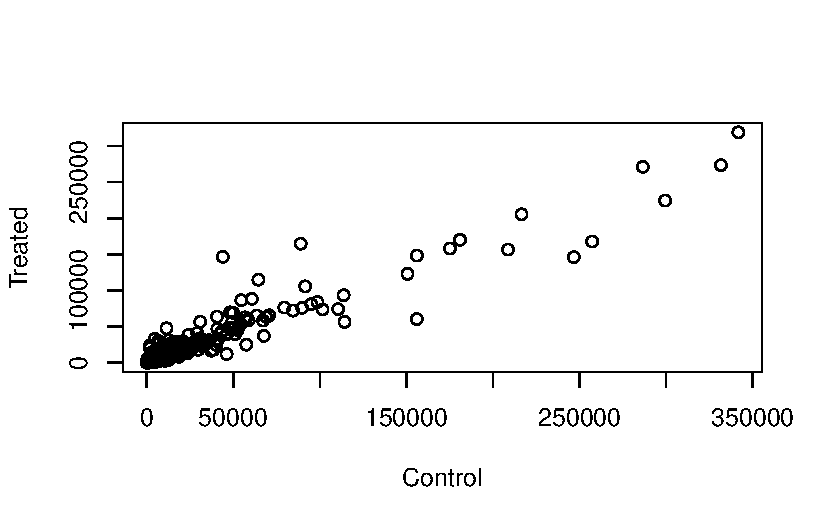
\includegraphics{12writeup_files/figure-pdf/unnamed-chunk-9-1.pdf}

}

\end{figure}

Q5B. What geom?() function would you use to create a ggplot out of this
data?

geom\_point()

Q6. What argument to plot() allows you to plot both axes on a log scale?

log=xy

\begin{Shaded}
\begin{Highlighting}[]
\FunctionTok{plot}\NormalTok{(meancounts[,}\DecValTok{1}\NormalTok{],meancounts[,}\DecValTok{2}\NormalTok{], }\AttributeTok{log =} \StringTok{"xy"}\NormalTok{,  }\AttributeTok{xlab=}\StringTok{"Control"}\NormalTok{, }\AttributeTok{ylab=}\StringTok{"Treated"}\NormalTok{)}
\end{Highlighting}
\end{Shaded}

\begin{verbatim}
Warning in xy.coords(x, y, xlabel, ylabel, log): 15032 x values <= 0 omitted
from logarithmic plot
\end{verbatim}

\begin{verbatim}
Warning in xy.coords(x, y, xlabel, ylabel, log): 15281 y values <= 0 omitted
from logarithmic plot
\end{verbatim}

\begin{figure}[H]

{\centering 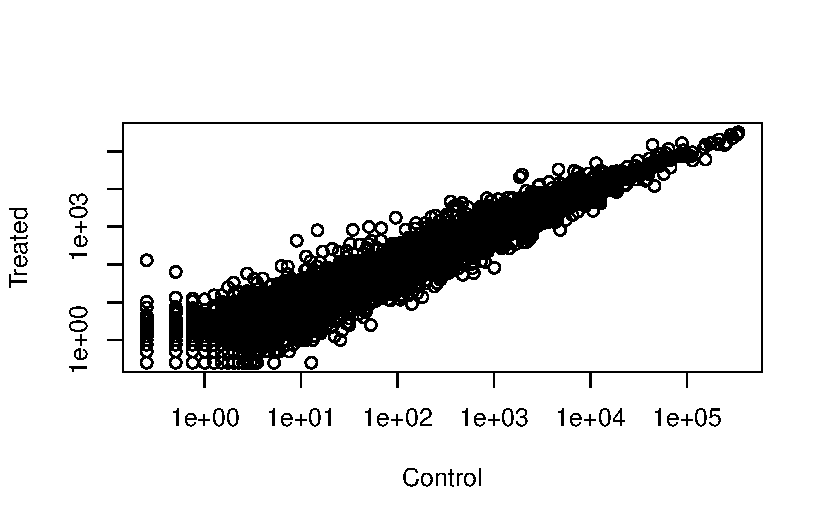
\includegraphics{12writeup_files/figure-pdf/unnamed-chunk-10-1.pdf}

}

\end{figure}

\begin{Shaded}
\begin{Highlighting}[]
\CommentTok{\#calculate log2foldchange and add it to meancounts dataframe}
\NormalTok{meancounts}\SpecialCharTok{$}\NormalTok{log2fc }\OtherTok{\textless{}{-}} \FunctionTok{log2}\NormalTok{(meancounts[,}\StringTok{"treated.mean"}\NormalTok{]}\SpecialCharTok{/}\NormalTok{meancounts[,}\StringTok{"control.mean"}\NormalTok{])}
\FunctionTok{head}\NormalTok{(meancounts)}
\end{Highlighting}
\end{Shaded}

\begin{verbatim}
                control.mean treated.mean      log2fc
ENSG00000000003       900.75       658.00 -0.45303916
ENSG00000000005         0.00         0.00         NaN
ENSG00000000419       520.50       546.00  0.06900279
ENSG00000000457       339.75       316.50 -0.10226805
ENSG00000000460        97.25        78.75 -0.30441833
ENSG00000000938         0.75         0.00        -Inf
\end{verbatim}

\begin{Shaded}
\begin{Highlighting}[]
\DocumentationTok{\#\#filtering out NaN/zero and negative infinity results}
\NormalTok{zero.vals }\OtherTok{\textless{}{-}} \FunctionTok{which}\NormalTok{(meancounts[,}\DecValTok{1}\SpecialCharTok{:}\DecValTok{2}\NormalTok{]}\SpecialCharTok{==}\DecValTok{0}\NormalTok{, }\AttributeTok{arr.ind=}\ConstantTok{TRUE}\NormalTok{)}

\NormalTok{to.rm }\OtherTok{\textless{}{-}} \FunctionTok{unique}\NormalTok{(zero.vals[,}\DecValTok{1}\NormalTok{])}
\NormalTok{mycounts }\OtherTok{\textless{}{-}}\NormalTok{ meancounts[}\SpecialCharTok{{-}}\NormalTok{to.rm,]}
\FunctionTok{head}\NormalTok{(mycounts)}
\end{Highlighting}
\end{Shaded}

\begin{verbatim}
                control.mean treated.mean      log2fc
ENSG00000000003       900.75       658.00 -0.45303916
ENSG00000000419       520.50       546.00  0.06900279
ENSG00000000457       339.75       316.50 -0.10226805
ENSG00000000460        97.25        78.75 -0.30441833
ENSG00000000971      5219.00      6687.50  0.35769358
ENSG00000001036      2327.00      1785.75 -0.38194109
\end{verbatim}

Q7. arr.ind will have which() return values that match the given value,
in this case: 0. Which will be looking at both rows and columns. Since
we don't want any values with 0 in the gene row, the unique function
will prevent a certain entry from being counted twice if it also has a 0
value in it's column.

\begin{Shaded}
\begin{Highlighting}[]
\NormalTok{up.ind }\OtherTok{\textless{}{-}}\NormalTok{ mycounts}\SpecialCharTok{$}\NormalTok{log2fc }\SpecialCharTok{\textgreater{}} \DecValTok{2}
\NormalTok{down.ind }\OtherTok{\textless{}{-}}\NormalTok{ mycounts}\SpecialCharTok{$}\NormalTok{log2fc }\SpecialCharTok{\textless{}}\NormalTok{ (}\SpecialCharTok{{-}}\DecValTok{2}\NormalTok{)}
\end{Highlighting}
\end{Shaded}

\begin{Shaded}
\begin{Highlighting}[]
\FunctionTok{which}\NormalTok{(up.ind, }\AttributeTok{arr.ind=}\ConstantTok{TRUE}\NormalTok{)}
\end{Highlighting}
\end{Shaded}

\begin{verbatim}
  [1]    59   149   203   290   338   344   576  1048  1055  1196  1618  1680
 [13]  1781  1939  1981  2038  2050  2118  2355  2358  2443  2514  2528  2599
 [25]  2686  3186  3265  3459  3548  3788  3836  4052  4128  4129  4244  4453
 [37]  4567  4659  4899  5124  5180  5181  5290  5386  5423  5484  5496  5498
 [49]  5584  5725  5964  6055  6167  6246  6277  6288  6364  6453  6518  6553
 [61]  6636  6869  6959  7034  7107  7108  7115  7183  7306  7348  7369  7422
 [73]  7617  7790  7913  7970  7989  8330  8365  8396  8530  8706  8714  8723
 [85]  8729  8741  8934  9175  9176  9213  9215  9270  9297  9392  9608  9753
 [97]  9828  9924  9940  9968  9971 10079 10146 10174 10229 10234 10515 10577
[109] 10631 10790 10955 10981 11019 11143 11177 11215 11341 11497 11520 11650
[121] 11798 11899 12087 12153 12237 12254 12269 12365 12637 12742 12828 12894
[133] 12922 12952 13071 13363 13426 13604 13813 13822 13832 13833 13851 13938
[145] 14099 14140 14151 14419 14472 14493 14519 14700 14820 14908 15111 15511
[157] 15526 15564 15567 15675 15766 15807 16310 16341 16361 16365 16415 16416
[169] 16421 16494 16630 16631 16638 16725 16929 16996 17115 17132 17206 17211
[181] 17285 17318 17332 17338 17357 17385 17485 17530 17550 17779 17918 17996
[193] 18061 18120 18163 18186 18246 18456 18493 18576 18650 18744 18839 18914
[205] 18960 19045 19052 19078 19129 19139 19150 19296 19297 19462 19530 19550
[217] 19666 19803 19915 20073 20183 20214 20314 20374 20384 20432 20445 20465
[229] 20553 20668 20766 20771 20774 20984 21093 21113 21119 21189 21190 21216
[241] 21266 21283 21317 21321 21391 21403 21409 21454 21544 21603
\end{verbatim}

\begin{Shaded}
\begin{Highlighting}[]
\FunctionTok{which}\NormalTok{(down.ind, }\AttributeTok{arr.ind=}\ConstantTok{TRUE}\NormalTok{)}
\end{Highlighting}
\end{Shaded}

\begin{verbatim}
  [1]   341   365   418   443   451   623   624   662   684   825   925  1124
 [13]  1142  1234  1238  1315  1351  1518  1551  1576  1623  1887  1911  1928
 [25]  1965  1974  2131  2245  2342  2375  2670  3015  3020  3091  3279  3320
 [37]  3332  3334  3355  3419  3794  3899  4001  4108  4286  4288  4331  4348
 [49]  4504  4605  4906  4933  4984  5009  5015  5053  5067  5154  5282  5320
 [61]  5397  5501  5518  5525  5535  5550  5555  5608  5684  5689  5724  5749
 [73]  5756  5779  5811  5873  5890  5904  5950  6073  6116  6293  6310  6370
 [85]  6504  6533  6684  6766  7000  7150  7189  7332  7396  7438  7521  7609
 [97]  7627  7858  7869  7936  8003  8013  8049  8052  8081  8114  8210  8212
[109]  8237  8407  8492  8501  8653  8667  8762  8875  9043  9189  9199  9274
[121]  9457  9600  9628  9807  9843  9853  9859  9983  9998 10020 10040 10176
[133] 10272 10361 10371 10487 10495 10526 10569 10586 10779 11138 11147 11159
[145] 11204 11237 11243 11332 11345 11417 11424 11436 11642 11710 11769 11848
[157] 12032 12240 12290 12395 12456 12466 12520 12549 12566 12618 12640 12671
[169] 12678 12687 12741 12826 12915 12964 13027 13193 13197 13211 13230 13324
[181] 13340 13348 13408 13410 13451 13464 13473 13484 13627 13677 13682 13812
[193] 13991 14033 14207 14226 14239 14285 14336 14350 14380 14406 14544 14628
[205] 14666 14720 14898 15147 15275 15282 15325 15388 15406 15420 15492 15655
[217] 15677 15731 15759 15787 15789 15840 15981 16063 16144 16234 16266 16283
[229] 16318 16343 16371 16395 16500 16502 16662 16709 16860 16876 16932 16949
[241] 16976 17024 17043 17069 17121 17162 17168 17196 17259 17326 17327 17344
[253] 17488 17543 17546 17587 17652 17667 17682 17709 17745 17808 17931 17932
[265] 17944 17957 18018 18051 18059 18197 18210 18299 18482 18490 18519 18521
[277] 18546 18578 18582 18618 18652 18763 18785 18812 18834 18841 18922 18968
[289] 19064 19094 19114 19187 19228 19243 19246 19270 19302 19311 19338 19347
[301] 19363 19443 19499 19551 19554 19613 19616 19654 19669 19801 19813 19814
[313] 19830 19890 19959 19976 20018 20074 20078 20096 20114 20128 20138 20233
[325] 20242 20254 20258 20270 20273 20277 20390 20404 20413 20434 20480 20483
[337] 20543 20559 20561 20599 20624 20631 20698 20709 20809 20813 20821 20894
[349] 20969 21009 21084 21118 21148 21154 21188 21249 21280 21335 21371 21416
[361] 21621 21627 21669 21673 21713 21744 21764
\end{verbatim}

Q8. How many up regulated genes? 250

Q9. How mayn downregulated genes? 367

Q10. Can we trust these results? No.~We have not been able to test the
results for statistic significance.

\begin{Shaded}
\begin{Highlighting}[]
\FunctionTok{library}\NormalTok{(DESeq2)}
\FunctionTok{citation}\NormalTok{(}\StringTok{"DESeq2"}\NormalTok{)}
\end{Highlighting}
\end{Shaded}

\begin{verbatim}
To cite package 'DESeq2' in publications use:

  Love, M.I., Huber, W., Anders, S. Moderated estimation of fold change
  and dispersion for RNA-seq data with DESeq2 Genome Biology 15(12):550
  (2014)

A BibTeX entry for LaTeX users is

  @Article{,
    title = {Moderated estimation of fold change and dispersion for RNA-seq data with DESeq2},
    author = {Michael I. Love and Wolfgang Huber and Simon Anders},
    year = {2014},
    journal = {Genome Biology},
    doi = {10.1186/s13059-014-0550-8},
    volume = {15},
    issue = {12},
    pages = {550},
  }
\end{verbatim}

\begin{Shaded}
\begin{Highlighting}[]
\NormalTok{dds }\OtherTok{\textless{}{-}} \FunctionTok{DESeqDataSetFromMatrix}\NormalTok{(}\AttributeTok{countData=}\NormalTok{counts, }\AttributeTok{colData=}\NormalTok{metadata, }\AttributeTok{design=}\SpecialCharTok{\textasciitilde{}}\NormalTok{dex)}
\end{Highlighting}
\end{Shaded}

\begin{verbatim}
converting counts to integer mode
\end{verbatim}

\begin{verbatim}
Warning in DESeqDataSet(se, design = design, ignoreRank): some variables in
design formula are characters, converting to factors
\end{verbatim}

\begin{Shaded}
\begin{Highlighting}[]
\NormalTok{dds }\OtherTok{\textless{}{-}} \FunctionTok{DESeq}\NormalTok{(dds)}
\end{Highlighting}
\end{Shaded}

\begin{verbatim}
estimating size factors
\end{verbatim}

\begin{verbatim}
estimating dispersions
\end{verbatim}

\begin{verbatim}
gene-wise dispersion estimates
\end{verbatim}

\begin{verbatim}
mean-dispersion relationship
\end{verbatim}

\begin{verbatim}
final dispersion estimates
\end{verbatim}

\begin{verbatim}
fitting model and testing
\end{verbatim}

\begin{Shaded}
\begin{Highlighting}[]
\NormalTok{res }\OtherTok{\textless{}{-}} \FunctionTok{results}\NormalTok{(dds)}
\NormalTok{res}
\end{Highlighting}
\end{Shaded}

\begin{verbatim}
log2 fold change (MLE): dex treated vs control 
Wald test p-value: dex treated vs control 
DataFrame with 38694 rows and 6 columns
                 baseMean log2FoldChange     lfcSE      stat    pvalue
                <numeric>      <numeric> <numeric> <numeric> <numeric>
ENSG00000000003  747.1942     -0.3507030  0.168246 -2.084470 0.0371175
ENSG00000000005    0.0000             NA        NA        NA        NA
ENSG00000000419  520.1342      0.2061078  0.101059  2.039475 0.0414026
ENSG00000000457  322.6648      0.0245269  0.145145  0.168982 0.8658106
ENSG00000000460   87.6826     -0.1471420  0.257007 -0.572521 0.5669691
...                   ...            ...       ...       ...       ...
ENSG00000283115  0.000000             NA        NA        NA        NA
ENSG00000283116  0.000000             NA        NA        NA        NA
ENSG00000283119  0.000000             NA        NA        NA        NA
ENSG00000283120  0.974916      -0.668258   1.69456 -0.394354  0.693319
ENSG00000283123  0.000000             NA        NA        NA        NA
                     padj
                <numeric>
ENSG00000000003  0.163035
ENSG00000000005        NA
ENSG00000000419  0.176032
ENSG00000000457  0.961694
ENSG00000000460  0.815849
...                   ...
ENSG00000283115        NA
ENSG00000283116        NA
ENSG00000283119        NA
ENSG00000283120        NA
ENSG00000283123        NA
\end{verbatim}

\begin{Shaded}
\begin{Highlighting}[]
\NormalTok{res2 }\OtherTok{\textless{}{-}} \FunctionTok{as.data.frame}\NormalTok{(res)}

\FunctionTok{View}\NormalTok{(res2)}
\end{Highlighting}
\end{Shaded}

\begin{Shaded}
\begin{Highlighting}[]
\FunctionTok{summary}\NormalTok{(res)}
\end{Highlighting}
\end{Shaded}

\begin{verbatim}

out of 25258 with nonzero total read count
adjusted p-value < 0.1
LFC > 0 (up)       : 1563, 6.2%
LFC < 0 (down)     : 1188, 4.7%
outliers [1]       : 142, 0.56%
low counts [2]     : 9971, 39%
(mean count < 10)
[1] see 'cooksCutoff' argument of ?results
[2] see 'independentFiltering' argument of ?results
\end{verbatim}

\begin{Shaded}
\begin{Highlighting}[]
\NormalTok{res05 }\OtherTok{\textless{}{-}} \FunctionTok{results}\NormalTok{(dds, }\AttributeTok{alpha=}\FloatTok{0.05}\NormalTok{)}
\FunctionTok{summary}\NormalTok{(res05)}
\end{Highlighting}
\end{Shaded}

\begin{verbatim}

out of 25258 with nonzero total read count
adjusted p-value < 0.05
LFC > 0 (up)       : 1236, 4.9%
LFC < 0 (down)     : 933, 3.7%
outliers [1]       : 142, 0.56%
low counts [2]     : 9033, 36%
(mean count < 6)
[1] see 'cooksCutoff' argument of ?results
[2] see 'independentFiltering' argument of ?results
\end{verbatim}

\begin{Shaded}
\begin{Highlighting}[]
\FunctionTok{library}\NormalTok{(}\StringTok{"AnnotationDbi"}\NormalTok{)}
\FunctionTok{library}\NormalTok{(}\StringTok{"org.Hs.eg.db"}\NormalTok{)}
\end{Highlighting}
\end{Shaded}

\begin{verbatim}
\end{verbatim}

\begin{Shaded}
\begin{Highlighting}[]
\FunctionTok{columns}\NormalTok{(org.Hs.eg.db)}
\end{Highlighting}
\end{Shaded}

\begin{verbatim}
 [1] "ACCNUM"       "ALIAS"        "ENSEMBL"      "ENSEMBLPROT"  "ENSEMBLTRANS"
 [6] "ENTREZID"     "ENZYME"       "EVIDENCE"     "EVIDENCEALL"  "GENENAME"    
[11] "GENETYPE"     "GO"           "GOALL"        "IPI"          "MAP"         
[16] "OMIM"         "ONTOLOGY"     "ONTOLOGYALL"  "PATH"         "PFAM"        
[21] "PMID"         "PROSITE"      "REFSEQ"       "SYMBOL"       "UCSCKG"      
[26] "UNIPROT"     
\end{verbatim}

\begin{Shaded}
\begin{Highlighting}[]
\CommentTok{\# adding columns to results table with mapIds}
\NormalTok{res}\SpecialCharTok{$}\NormalTok{symbol }\OtherTok{\textless{}{-}} \FunctionTok{mapIds}\NormalTok{(org.Hs.eg.db,}
                     \AttributeTok{keys=}\FunctionTok{row.names}\NormalTok{(res), }\CommentTok{\# Our genenames}
                     \AttributeTok{keytype=}\StringTok{"ENSEMBL"}\NormalTok{,   }\CommentTok{\# The format of our genenames}
                     \AttributeTok{column=}\StringTok{"SYMBOL"}\NormalTok{,     }\CommentTok{\# The new format we want to add}
                     \AttributeTok{multiVals=}\StringTok{"first"}\NormalTok{)}
\end{Highlighting}
\end{Shaded}

\begin{verbatim}
'select()' returned 1:many mapping between keys and columns
\end{verbatim}

\begin{Shaded}
\begin{Highlighting}[]
\FunctionTok{head}\NormalTok{(res)}
\end{Highlighting}
\end{Shaded}

\begin{verbatim}
log2 fold change (MLE): dex treated vs control 
Wald test p-value: dex treated vs control 
DataFrame with 6 rows and 7 columns
                  baseMean log2FoldChange     lfcSE      stat    pvalue
                 <numeric>      <numeric> <numeric> <numeric> <numeric>
ENSG00000000003 747.194195     -0.3507030  0.168246 -2.084470 0.0371175
ENSG00000000005   0.000000             NA        NA        NA        NA
ENSG00000000419 520.134160      0.2061078  0.101059  2.039475 0.0414026
ENSG00000000457 322.664844      0.0245269  0.145145  0.168982 0.8658106
ENSG00000000460  87.682625     -0.1471420  0.257007 -0.572521 0.5669691
ENSG00000000938   0.319167     -1.7322890  3.493601 -0.495846 0.6200029
                     padj      symbol
                <numeric> <character>
ENSG00000000003  0.163035      TSPAN6
ENSG00000000005        NA        TNMD
ENSG00000000419  0.176032        DPM1
ENSG00000000457  0.961694       SCYL3
ENSG00000000460  0.815849       FIRRM
ENSG00000000938        NA         FGR
\end{verbatim}

\begin{Shaded}
\begin{Highlighting}[]
\NormalTok{res}\SpecialCharTok{$}\NormalTok{entrez }\OtherTok{\textless{}{-}} \FunctionTok{mapIds}\NormalTok{(org.Hs.eg.db,}
                     \AttributeTok{keys=}\FunctionTok{row.names}\NormalTok{(res),}
                     \AttributeTok{column=}\StringTok{"ENTREZID"}\NormalTok{,}
                     \AttributeTok{keytype=}\StringTok{"ENSEMBL"}\NormalTok{,}
                     \AttributeTok{multiVals=}\StringTok{"first"}\NormalTok{)}
\end{Highlighting}
\end{Shaded}

\begin{verbatim}
'select()' returned 1:many mapping between keys and columns
\end{verbatim}

\begin{Shaded}
\begin{Highlighting}[]
\NormalTok{res}\SpecialCharTok{$}\NormalTok{uniprot }\OtherTok{\textless{}{-}} \FunctionTok{mapIds}\NormalTok{(org.Hs.eg.db,}
                     \AttributeTok{keys=}\FunctionTok{row.names}\NormalTok{(res),}
                     \AttributeTok{column=}\StringTok{"UNIPROT"}\NormalTok{,}
                     \AttributeTok{keytype=}\StringTok{"ENSEMBL"}\NormalTok{,}
                     \AttributeTok{multiVals=}\StringTok{"first"}\NormalTok{)}
\end{Highlighting}
\end{Shaded}

\begin{verbatim}
'select()' returned 1:many mapping between keys and columns
\end{verbatim}

\begin{Shaded}
\begin{Highlighting}[]
\NormalTok{res}\SpecialCharTok{$}\NormalTok{genename }\OtherTok{\textless{}{-}} \FunctionTok{mapIds}\NormalTok{(org.Hs.eg.db,}
                     \AttributeTok{keys=}\FunctionTok{row.names}\NormalTok{(res),}
                     \AttributeTok{column=}\StringTok{"GENENAME"}\NormalTok{,}
                     \AttributeTok{keytype=}\StringTok{"ENSEMBL"}\NormalTok{,}
                     \AttributeTok{multiVals=}\StringTok{"first"}\NormalTok{)}
\end{Highlighting}
\end{Shaded}

\begin{verbatim}
'select()' returned 1:many mapping between keys and columns
\end{verbatim}

\begin{Shaded}
\begin{Highlighting}[]
\FunctionTok{head}\NormalTok{(res)}
\end{Highlighting}
\end{Shaded}

\begin{verbatim}
log2 fold change (MLE): dex treated vs control 
Wald test p-value: dex treated vs control 
DataFrame with 6 rows and 10 columns
                  baseMean log2FoldChange     lfcSE      stat    pvalue
                 <numeric>      <numeric> <numeric> <numeric> <numeric>
ENSG00000000003 747.194195     -0.3507030  0.168246 -2.084470 0.0371175
ENSG00000000005   0.000000             NA        NA        NA        NA
ENSG00000000419 520.134160      0.2061078  0.101059  2.039475 0.0414026
ENSG00000000457 322.664844      0.0245269  0.145145  0.168982 0.8658106
ENSG00000000460  87.682625     -0.1471420  0.257007 -0.572521 0.5669691
ENSG00000000938   0.319167     -1.7322890  3.493601 -0.495846 0.6200029
                     padj      symbol      entrez     uniprot
                <numeric> <character> <character> <character>
ENSG00000000003  0.163035      TSPAN6        7105  A0A024RCI0
ENSG00000000005        NA        TNMD       64102      Q9H2S6
ENSG00000000419  0.176032        DPM1        8813      O60762
ENSG00000000457  0.961694       SCYL3       57147      Q8IZE3
ENSG00000000460  0.815849       FIRRM       55732  A0A024R922
ENSG00000000938        NA         FGR        2268      P09769
                              genename
                           <character>
ENSG00000000003          tetraspanin 6
ENSG00000000005            tenomodulin
ENSG00000000419 dolichyl-phosphate m..
ENSG00000000457 SCY1 like pseudokina..
ENSG00000000460 FIGNL1 interacting r..
ENSG00000000938 FGR proto-oncogene, ..
\end{verbatim}

\begin{Shaded}
\begin{Highlighting}[]
\CommentTok{\#arrange and view results by p{-}value}
\NormalTok{ord }\OtherTok{\textless{}{-}} \FunctionTok{order}\NormalTok{( res}\SpecialCharTok{$}\NormalTok{padj )}
\CommentTok{\#View(res[ord,])}
\FunctionTok{head}\NormalTok{(res[ord,])}
\end{Highlighting}
\end{Shaded}

\begin{verbatim}
log2 fold change (MLE): dex treated vs control 
Wald test p-value: dex treated vs control 
DataFrame with 6 rows and 10 columns
                 baseMean log2FoldChange     lfcSE      stat      pvalue
                <numeric>      <numeric> <numeric> <numeric>   <numeric>
ENSG00000152583   954.771        4.36836 0.2371268   18.4220 8.74490e-76
ENSG00000179094   743.253        2.86389 0.1755693   16.3120 8.10784e-60
ENSG00000116584  2277.913       -1.03470 0.0650984  -15.8944 6.92855e-57
ENSG00000189221  2383.754        3.34154 0.2124058   15.7319 9.14433e-56
ENSG00000120129  3440.704        2.96521 0.2036951   14.5571 5.26424e-48
ENSG00000148175 13493.920        1.42717 0.1003890   14.2164 7.25128e-46
                       padj      symbol      entrez     uniprot
                  <numeric> <character> <character> <character>
ENSG00000152583 1.32441e-71     SPARCL1        8404  A0A024RDE1
ENSG00000179094 6.13966e-56        PER1        5187      O15534
ENSG00000116584 3.49776e-53     ARHGEF2        9181      Q92974
ENSG00000189221 3.46227e-52        MAOA        4128      P21397
ENSG00000120129 1.59454e-44       DUSP1        1843      B4DU40
ENSG00000148175 1.83034e-42        STOM        2040      F8VSL7
                              genename
                           <character>
ENSG00000152583           SPARC like 1
ENSG00000179094 period circadian reg..
ENSG00000116584 Rho/Rac guanine nucl..
ENSG00000189221    monoamine oxidase A
ENSG00000120129 dual specificity pho..
ENSG00000148175               stomatin
\end{verbatim}

\begin{Shaded}
\begin{Highlighting}[]
\FunctionTok{write.csv}\NormalTok{(res[ord,], }\StringTok{"deseq\_results.csv"}\NormalTok{)}
\end{Highlighting}
\end{Shaded}

\begin{Shaded}
\begin{Highlighting}[]
\FunctionTok{plot}\NormalTok{(res}\SpecialCharTok{$}\NormalTok{log2FoldChange, }\SpecialCharTok{{-}}\FunctionTok{log}\NormalTok{(res}\SpecialCharTok{$}\NormalTok{padj), }
      \AttributeTok{xlab=}\StringTok{"Log2(FoldChange)"}\NormalTok{,}
      \AttributeTok{ylab=}\StringTok{"{-}Log(P{-}value)"}\NormalTok{)}
\end{Highlighting}
\end{Shaded}

\begin{figure}[H]

{\centering 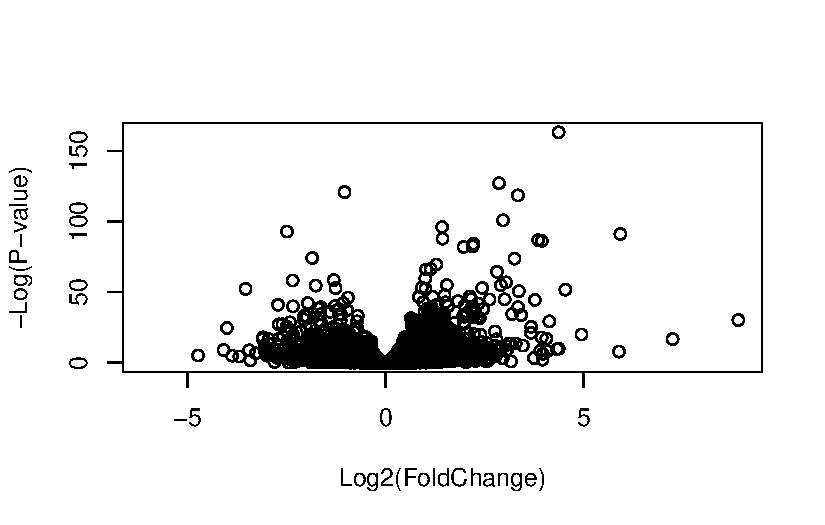
\includegraphics{12writeup_files/figure-pdf/unnamed-chunk-29-1.pdf}

}

\end{figure}

\begin{Shaded}
\begin{Highlighting}[]
\FunctionTok{plot}\NormalTok{( res}\SpecialCharTok{$}\NormalTok{log2FoldChange,  }\SpecialCharTok{{-}}\FunctionTok{log}\NormalTok{(res}\SpecialCharTok{$}\NormalTok{padj), }
 \AttributeTok{ylab=}\StringTok{"{-}Log(P{-}value)"}\NormalTok{, }\AttributeTok{xlab=}\StringTok{"Log2(FoldChange)"}\NormalTok{)}

\CommentTok{\# Add some cut{-}off lines}
\FunctionTok{abline}\NormalTok{(}\AttributeTok{v=}\FunctionTok{c}\NormalTok{(}\SpecialCharTok{{-}}\DecValTok{2}\NormalTok{,}\DecValTok{2}\NormalTok{), }\AttributeTok{col=}\StringTok{"darkgray"}\NormalTok{, }\AttributeTok{lty=}\DecValTok{2}\NormalTok{)}
\FunctionTok{abline}\NormalTok{(}\AttributeTok{h=}\SpecialCharTok{{-}}\FunctionTok{log}\NormalTok{(}\FloatTok{0.05}\NormalTok{), }\AttributeTok{col=}\StringTok{"darkgray"}\NormalTok{, }\AttributeTok{lty=}\DecValTok{2}\NormalTok{)}
\end{Highlighting}
\end{Shaded}

\begin{figure}[H]

{\centering 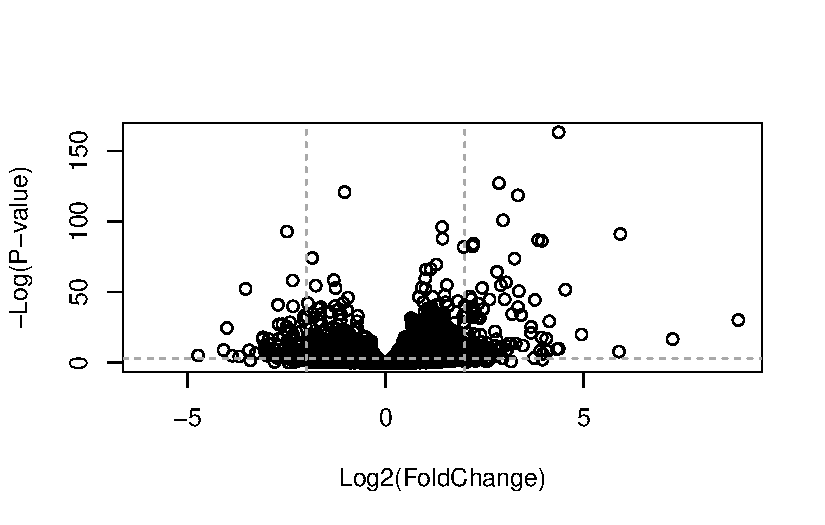
\includegraphics{12writeup_files/figure-pdf/unnamed-chunk-30-1.pdf}

}

\end{figure}

\begin{Shaded}
\begin{Highlighting}[]
\CommentTok{\# Setup our custom point color vector }
\NormalTok{mycols }\OtherTok{\textless{}{-}} \FunctionTok{rep}\NormalTok{(}\StringTok{"gray"}\NormalTok{, }\FunctionTok{nrow}\NormalTok{(res))}
\NormalTok{mycols[ }\FunctionTok{abs}\NormalTok{(res}\SpecialCharTok{$}\NormalTok{log2FoldChange) }\SpecialCharTok{\textgreater{}} \DecValTok{2}\NormalTok{ ]  }\OtherTok{\textless{}{-}} \StringTok{"red"} 

\NormalTok{inds }\OtherTok{\textless{}{-}}\NormalTok{ (res}\SpecialCharTok{$}\NormalTok{padj }\SpecialCharTok{\textless{}} \FloatTok{0.01}\NormalTok{) }\SpecialCharTok{\&}\NormalTok{ (}\FunctionTok{abs}\NormalTok{(res}\SpecialCharTok{$}\NormalTok{log2FoldChange) }\SpecialCharTok{\textgreater{}} \DecValTok{2}\NormalTok{ )}
\NormalTok{mycols[ inds ] }\OtherTok{\textless{}{-}} \StringTok{"blue"}

\CommentTok{\# Volcano plot with custom colors }
\FunctionTok{plot}\NormalTok{( res}\SpecialCharTok{$}\NormalTok{log2FoldChange,  }\SpecialCharTok{{-}}\FunctionTok{log}\NormalTok{(res}\SpecialCharTok{$}\NormalTok{padj), }
 \AttributeTok{col=}\NormalTok{mycols, }\AttributeTok{ylab=}\StringTok{"{-}Log(P{-}value)"}\NormalTok{, }\AttributeTok{xlab=}\StringTok{"Log2(FoldChange)"}\NormalTok{ )}

\CommentTok{\# Cut{-}off lines}
\FunctionTok{abline}\NormalTok{(}\AttributeTok{v=}\FunctionTok{c}\NormalTok{(}\SpecialCharTok{{-}}\DecValTok{2}\NormalTok{,}\DecValTok{2}\NormalTok{), }\AttributeTok{col=}\StringTok{"gray"}\NormalTok{, }\AttributeTok{lty=}\DecValTok{2}\NormalTok{)}
\FunctionTok{abline}\NormalTok{(}\AttributeTok{h=}\SpecialCharTok{{-}}\FunctionTok{log}\NormalTok{(}\FloatTok{0.1}\NormalTok{), }\AttributeTok{col=}\StringTok{"gray"}\NormalTok{, }\AttributeTok{lty=}\DecValTok{2}\NormalTok{)}
\end{Highlighting}
\end{Shaded}

\begin{figure}[H]

{\centering 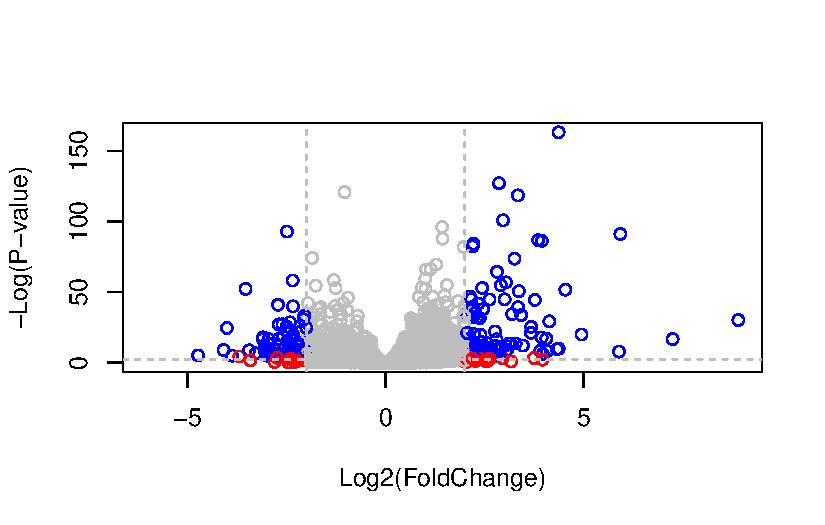
\includegraphics{12writeup_files/figure-pdf/unnamed-chunk-31-1.pdf}

}

\end{figure}

\begin{Shaded}
\begin{Highlighting}[]
\FunctionTok{library}\NormalTok{(EnhancedVolcano)}
\end{Highlighting}
\end{Shaded}

\begin{verbatim}
Loading required package: ggplot2
\end{verbatim}

\begin{verbatim}
Loading required package: ggrepel
\end{verbatim}

\begin{Shaded}
\begin{Highlighting}[]
\NormalTok{x }\OtherTok{\textless{}{-}} \FunctionTok{as.data.frame}\NormalTok{(res)}

\FunctionTok{EnhancedVolcano}\NormalTok{(x,}
    \AttributeTok{lab =}\NormalTok{ x}\SpecialCharTok{$}\NormalTok{symbol,}
    \AttributeTok{x =} \StringTok{\textquotesingle{}log2FoldChange\textquotesingle{}}\NormalTok{,}
    \AttributeTok{y =} \StringTok{\textquotesingle{}pvalue\textquotesingle{}}\NormalTok{)}
\end{Highlighting}
\end{Shaded}

\begin{figure}[H]

{\centering 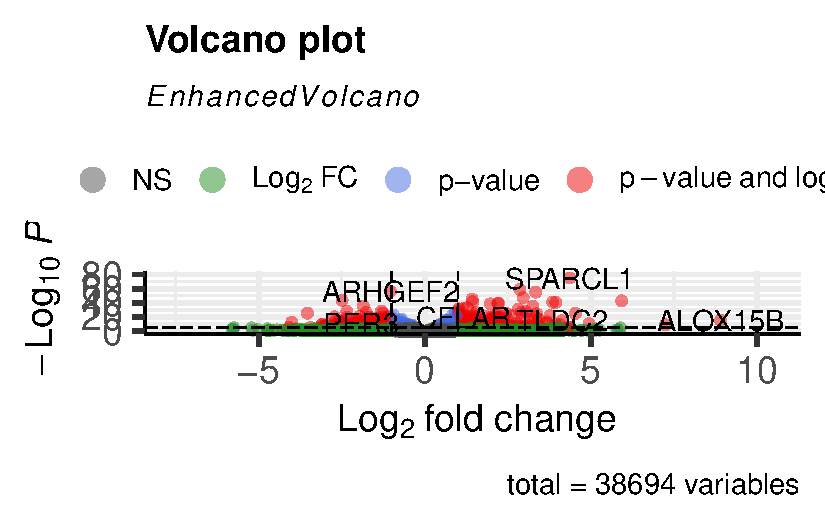
\includegraphics{12writeup_files/figure-pdf/unnamed-chunk-33-1.pdf}

}

\end{figure}

\begin{Shaded}
\begin{Highlighting}[]
\FunctionTok{library}\NormalTok{(pathview)}
\end{Highlighting}
\end{Shaded}

\begin{verbatim}
##############################################################################
Pathview is an open source software package distributed under GNU General
Public License version 3 (GPLv3). Details of GPLv3 is available at
http://www.gnu.org/licenses/gpl-3.0.html. Particullary, users are required to
formally cite the original Pathview paper (not just mention it) in publications
or products. For details, do citation("pathview") within R.

The pathview downloads and uses KEGG data. Non-academic uses may require a KEGG
license agreement (details at http://www.kegg.jp/kegg/legal.html).
##############################################################################
\end{verbatim}

\begin{Shaded}
\begin{Highlighting}[]
\FunctionTok{library}\NormalTok{(gage)}
\end{Highlighting}
\end{Shaded}

\begin{verbatim}
\end{verbatim}

\begin{Shaded}
\begin{Highlighting}[]
\FunctionTok{library}\NormalTok{(gageData)}
\end{Highlighting}
\end{Shaded}

\begin{Shaded}
\begin{Highlighting}[]
\FunctionTok{data}\NormalTok{(kegg.sets.hs)}

\CommentTok{\# Examine the first 2 pathways in this kegg set for humans}
\FunctionTok{head}\NormalTok{(kegg.sets.hs, }\DecValTok{2}\NormalTok{)}
\end{Highlighting}
\end{Shaded}

\begin{verbatim}
$`hsa00232 Caffeine metabolism`
[1] "10"   "1544" "1548" "1549" "1553" "7498" "9"   

$`hsa00983 Drug metabolism - other enzymes`
 [1] "10"     "1066"   "10720"  "10941"  "151531" "1548"   "1549"   "1551"  
 [9] "1553"   "1576"   "1577"   "1806"   "1807"   "1890"   "221223" "2990"  
[17] "3251"   "3614"   "3615"   "3704"   "51733"  "54490"  "54575"  "54576" 
[25] "54577"  "54578"  "54579"  "54600"  "54657"  "54658"  "54659"  "54963" 
[33] "574537" "64816"  "7083"   "7084"   "7172"   "7363"   "7364"   "7365"  
[41] "7366"   "7367"   "7371"   "7372"   "7378"   "7498"   "79799"  "83549" 
[49] "8824"   "8833"   "9"      "978"   
\end{verbatim}

\begin{Shaded}
\begin{Highlighting}[]
\NormalTok{foldchanges }\OtherTok{=}\NormalTok{ res}\SpecialCharTok{$}\NormalTok{log2FoldChange}
\FunctionTok{names}\NormalTok{(foldchanges) }\OtherTok{=}\NormalTok{ res}\SpecialCharTok{$}\NormalTok{entrez}
\FunctionTok{head}\NormalTok{(foldchanges)}
\end{Highlighting}
\end{Shaded}

\begin{verbatim}
       7105       64102        8813       57147       55732        2268 
-0.35070302          NA  0.20610777  0.02452695 -0.14714205 -1.73228897 
\end{verbatim}

\begin{Shaded}
\begin{Highlighting}[]
\CommentTok{\# Get the results}
\NormalTok{keggres }\OtherTok{=} \FunctionTok{gage}\NormalTok{(foldchanges, }\AttributeTok{gsets=}\NormalTok{kegg.sets.hs)}
\end{Highlighting}
\end{Shaded}

\begin{Shaded}
\begin{Highlighting}[]
\FunctionTok{attributes}\NormalTok{(keggres)}
\end{Highlighting}
\end{Shaded}

\begin{verbatim}
$names
[1] "greater" "less"    "stats"  
\end{verbatim}

\begin{Shaded}
\begin{Highlighting}[]
\CommentTok{\# Look at the first three down (less) pathways}
\FunctionTok{head}\NormalTok{(keggres}\SpecialCharTok{$}\NormalTok{less, }\DecValTok{3}\NormalTok{)}
\end{Highlighting}
\end{Shaded}

\begin{verbatim}
                                      p.geomean stat.mean        p.val
hsa05332 Graft-versus-host disease 0.0004250461 -3.473346 0.0004250461
hsa04940 Type I diabetes mellitus  0.0017820293 -3.002352 0.0017820293
hsa05310 Asthma                    0.0020045888 -3.009050 0.0020045888
                                        q.val set.size         exp1
hsa05332 Graft-versus-host disease 0.09053483       40 0.0004250461
hsa04940 Type I diabetes mellitus  0.14232581       42 0.0017820293
hsa05310 Asthma                    0.14232581       29 0.0020045888
\end{verbatim}

\begin{Shaded}
\begin{Highlighting}[]
\FunctionTok{pathview}\NormalTok{(}\AttributeTok{gene.data=}\NormalTok{foldchanges, }\AttributeTok{pathway.id=}\StringTok{"hsa05310"}\NormalTok{)}
\end{Highlighting}
\end{Shaded}

\begin{verbatim}
'select()' returned 1:1 mapping between keys and columns
\end{verbatim}

\begin{verbatim}
Info: Working in directory C:/Users/sutor/OneDrive/Desktop/bimm143/12bioconDESeq2
\end{verbatim}

\begin{verbatim}
Info: Writing image file hsa05310.pathview.png
\end{verbatim}



\end{document}
